\section{Infrastructure}

\subsection{Dardel}
\frame{
\frametitle{Dardel - an HPE Cray XE supercomputer}

\begin{alertblock}{}{\alert{CPU partition}}\end{alertblock}

\begin{columns}
\column{.6\textwidth}
  \begin{itemize}
    \item 2.279 petaFlops (Top500 Nov.2021)
    \item 554 CPU nodes
    \item Dual AMD EPYC$^{\rm TM}$ 64-core processors
    \item 256, 512, 1024, or 2048 GB memory
  \end{itemize}
\column{.4\textwidth}
  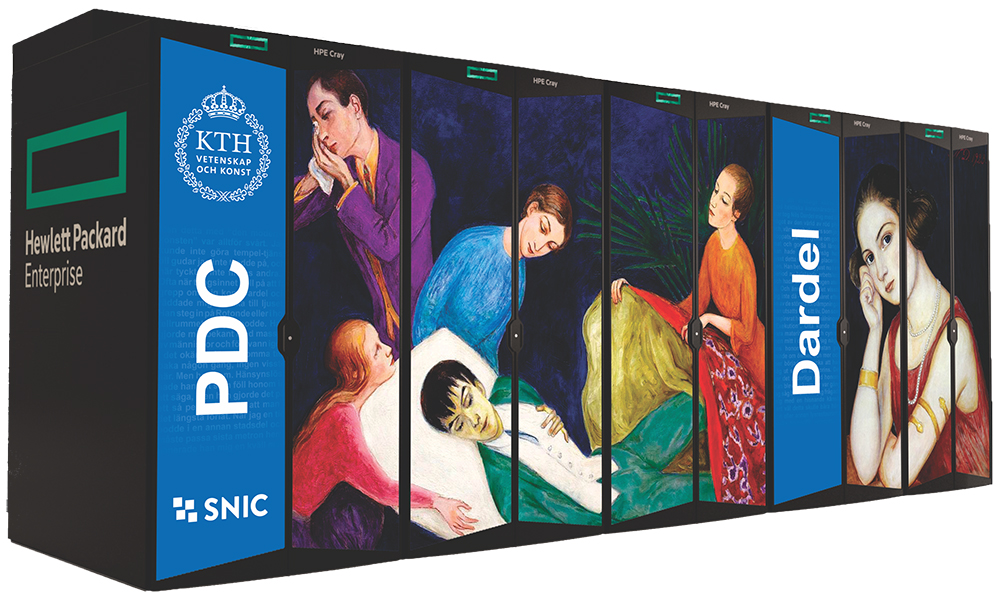
\includegraphics[width=\columnwidth]{dardel}
\end{columns}

\begin{alertblock}{}{\alert{GPU partition}}\end{alertblock}

\begin{columns}
\column{1.\textwidth}
  \begin{itemize}
    \item $56$ GPU nodes
    \item AMD EPYC$^{\rm TM}$ processor with 64 cores (under development)
    \item 512 GB memory
    \item four AMD Instinct$^{\rm TM}$ MI250X GPUs
  \end{itemize}
\end{columns}

}

\subsection*{File systems}
\frame{
\frametitle{File Systems}

\begin{block}{Lustre File System (\alert{Klemming})}
\begin{itemize}
 \item Open-source massively parallel distributed file system
 \item Optimized for handling data from many clients
 \item Total size is $12$ PB (12,000 TB)
 \item Home directory (25 GB, with backup)\\  {/cfs/klemming/home/[u]/[username]}
 \item Project directory \\  {/cfs/klemming/projects/snic/[projectname]}
 \item Scratch directory \\  {/cfs/klemming/scratch/[u]/[username]}
\end{itemize}
\end{block}

\footnotesize
\href{https://www.pdc.kth.se/support/documents/data\_management/klemming.html}{https://www.pdc.kth.se/support/documents/data\_management/klemming.html}

}

\frame{
\frametitle{File Systems}

\begin{itemize}
\item Good practice
    \begin{itemize}
    \item Minimize the number of I/O operations
    \item Avoid creating too many files
    \item Avoid creating directories with a large numbers of files
    \end{itemize}
\end{itemize}

\begin{itemize}
\item Bad practice
    \begin{itemize}
    \item Small reads
    \item Opening many files
    \item Seeking within a file to read a small piece of data
    \end{itemize}
\end{itemize}

}


\begin{frame}[fragile]
\frametitle{Access Control Lists}

\begin{exampleblock}{To view the access for a folder:}
\footnotesize
\begin{verbatim}
getfacl -a /cfs/klemming/home/u/user/test
\end{verbatim}
\end{exampleblock}

\begin{exampleblock}{The output looks like this:}
\footnotesize
\begin{verbatim}
# file: /cfs/klemming/home/u/user/test
# owner: me
# group: users
user::rwx
group::r-x
other::---
\end{verbatim}
\end{exampleblock}

\begin{exampleblock}{To grant the access to another user:}
\footnotesize
\begin{verbatim}
setfacl -m u:<uid>:r-x -R /cfs/klemming/home/u/user/test
\end{verbatim}
\end{exampleblock}

\begin{exampleblock}{To remove the access for another user:}
\footnotesize
\begin{verbatim}
setfacl -x u:<uid> -R /cfs/klemming/home/u/user/test
\end{verbatim}
\end{exampleblock}

\end{frame}



\frame<presentation:0>[noframenumbering]{
\frametitle{File System Access}
 \begin{tabular}{ccc}
   
  \cellcolor{kthLightGreen} \textbf{AFS} & 
  \cellcolor{kthLightBlue}{Beskow Compute Node} &
  \cellcolor{kthLightBlue}\textbf{CFS}\\
   
  \cellcolor{kthLightGreen} Andrew File System & 
  \cellcolor{kthLightGreen!50!kthLightBlue} Beskow Login Node &  
  \cellcolor{kthLightBlue} Lustre File System\\ 
  
  \cellcolor{kthLightGreen}~ &
  \cellcolor{kthLightGreen!50!kthLightBlue}~ &
  \cellcolor{kthLightBlue}~\\

  \cellcolor{kthLightGreen} & 
  \cellcolor{kthLightGreen!50!kthLightBlue} Tegner Compute Node &  
  \cellcolor{kthLightBlue} \scriptsize{\url {/cfs/klemming/ }\alert{\textbf{nobackup}}\url{/}} \\
  
  
  \cellcolor{kthLightGreen} \scriptsize{\url{/afs/pdc.kth.se/home/}} & 
  \cellcolor{kthLightGreen!50!kthLightBlue} Tegner Login Node &  
  \cellcolor{kthLightBlue} \scriptsize{\url{/[initial]/[username]}} \\

  \cellcolor{kthLightGreen} \scriptsize{\url{/[initial]/[username]}}  &
  \cellcolor{kthLightGreen} &
  \cellcolor{kthLightBlue} \\

  \cellcolor{kthLightGreen} & 
  \cellcolor{kthLightGreen} KTH (Linux) computer &  
  \cellcolor{kthLightBlue} \scriptsize{\url{/cfs/klemming/}\alert{\textbf{scratch}}\url{/}}\\
 
  \cellcolor{kthLightGreen} &
  \cellcolor{kthLightGreen} & 
  \cellcolor{kthLightBlue} \scriptsize{\url{/[initial]/[username]}}\\
   
  \cellcolor{kthLightGreen} & 
  \cellcolor{kthLightGreen} Laptop/Home computer &
  \cellcolor{kthLightBlue}
  \end{tabular}
}

\frame<presentation:0>[noframenumbering]{
\frametitle{File System Access}
 
\begin{tikzpicture}
\begin{scope}[transparency group]
\begin{scope}[blend mode=multiply]
  \coordinate (AFS) at (1,0);
  \coordinate (CFS) at (4,0);
  \coordinate (LARGE) at (9,0);
  %\node at (3,-1) {\alert{\textbf{AFS}}}; 
  \node[align=center,text width=3.1cm] at (2.5,1.5) {\textbf{\alert{Tegner Login Node}}};
  \node[align=center,text width=3.1cm] at (2.5,0) {\textbf{Tegner Compute Node}};
  \node[align=center,opacity=1,text width=1.5cm] at (2.5,-2) {\textbf{Beskow Login Node}};
  
  \node[align=center,text width=2cm] at (6,0) {\textbf{Beskow Compute Node}};
  
  \node[align=left,text width=2.3cm] at (0,2) {\textbf{KTH (Linux) computer}};
  \node[align=center,text width=2.5cm] at (-1,-1) {\textbf{Laptop/Home computer}};
  
  \filldraw[fill=kthLightBlue, draw=black,opacity=0.5,rounded corners=1mm] (AFS) \irregularcircle{3.5cm}{3mm};
  \filldraw[fill=kthLightGreen, draw=black,opacity=0.5,rounded corners=1mm] (CFS) \irregularcircle{3.5cm}{2mm};
\end{scope}
\end{scope}
\end{tikzpicture}

  
}
